% Editable source for clock_boundaries.pdf (pdflatex clock_boundaries.tex).
% Clock boundaries of the N83 one-target Tier 1 protocol. Widths are schematic, not to scale.
\documentclass[tikz,border=6pt]{standalone}
\usepackage[T1]{fontenc}
\usetikzlibrary{positioning,decorations.pathreplacing}
\begin{document}
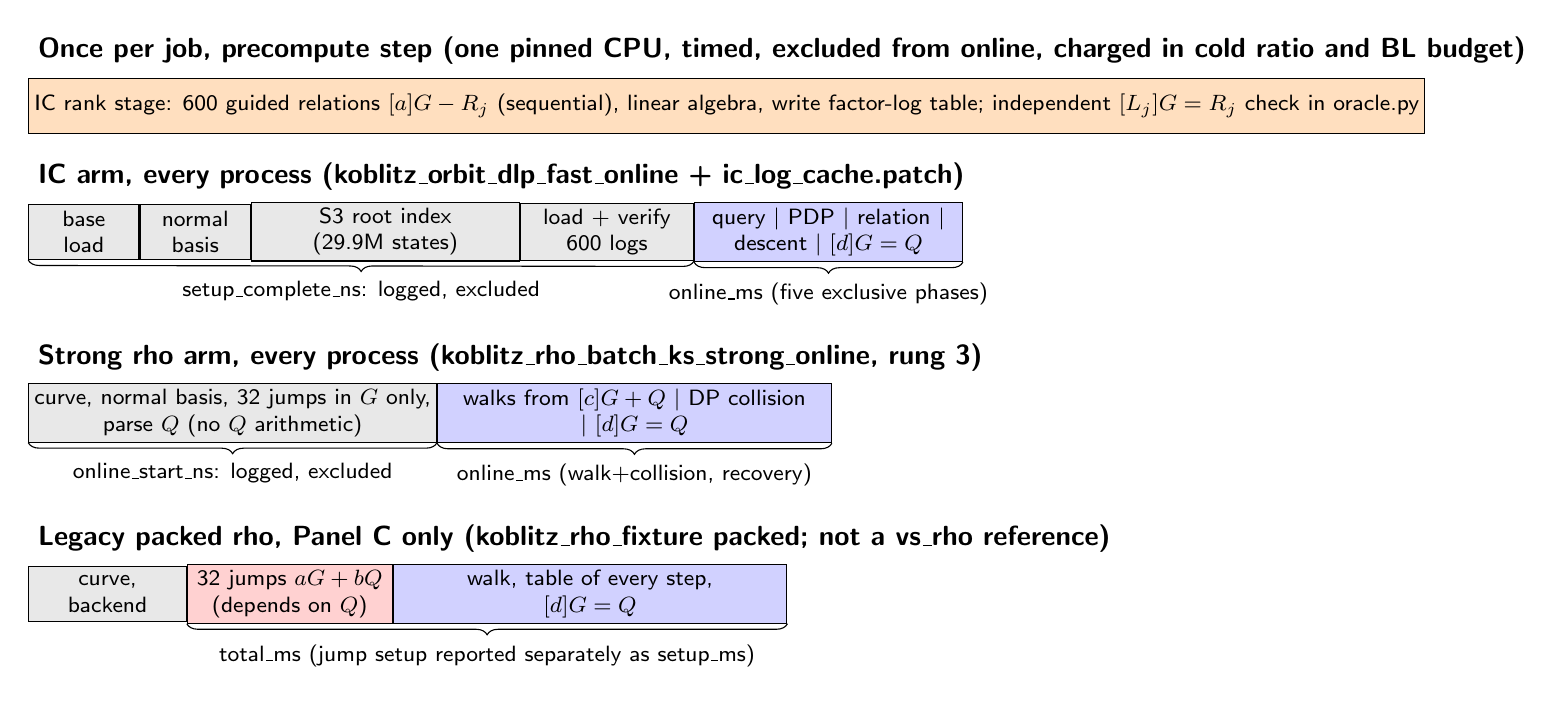
\begin{tikzpicture}[font=\sffamily\footnotesize,
  box/.style={draw,minimum height=7mm,inner sep=2pt,align=center},
  setup/.style={box,fill=gray!18},
  once/.style={box,fill=orange!25},
  online/.style={box,fill=blue!18},
  dep/.style={box,fill=red!18}]
\node[anchor=west,font=\sffamily\bfseries] at (0,4.9) {Once per job, precompute step (one pinned CPU, timed, excluded from online, charged in cold ratio and BL budget)};
\node[once,minimum width=118mm,anchor=west] (rank) at (0,4.2) {IC rank stage: 600 guided relations $[a]G-R_j$ (sequential), linear algebra, write factor-log table; independent $[L_j]G=R_j$ check in oracle.py};
\node[anchor=west,font=\sffamily\bfseries] at (0,3.3) {IC arm, every process (koblitz\_orbit\_dlp\_fast\_online + ic\_log\_cache.patch)};
\node[setup,minimum width=14mm,anchor=west] (b) at (0,2.6) {base\\load};
\node[setup,minimum width=14mm,right=0mm of b] (nb) {normal\\basis};
\node[setup,minimum width=34mm,right=0mm of nb] (ix) {S3 root index\\(29.9M states)};
\node[setup,minimum width=22mm,right=0mm of ix] (lg) {load + verify\\600 logs};
\node[online,minimum width=34mm,right=0mm of lg] (ic) {query $|$ PDP $|$ relation $|$\\descent $|$ $[d]G=Q$};
\draw[decorate,decoration={brace,mirror,amplitude=4pt}] (b.south west) -- (lg.south east) node[midway,below=4pt]{setup\_complete\_ns: logged, excluded};
\draw[decorate,decoration={brace,mirror,amplitude=4pt}] (ic.south west) -- (ic.south east) node[midway,below=4pt]{online\_ms (five exclusive phases)};
\node[anchor=west,font=\sffamily\bfseries] at (0,1.0) {Strong rho arm, every process (koblitz\_rho\_batch\_ks\_strong\_online, rung 3)};
\node[setup,minimum width=46mm,anchor=west] (rs) at (0,0.3) {curve, normal basis, 32 jumps in $G$ only,\\parse $Q$ (no $Q$ arithmetic)};
\node[online,minimum width=50mm,right=0mm of rs] (rw) {walks from $[c]G+Q$ $|$ DP collision\\$|$ $[d]G=Q$};
\draw[decorate,decoration={brace,mirror,amplitude=4pt}] (rs.south west) -- (rs.south east) node[midway,below=4pt]{online\_start\_ns: logged, excluded};
\draw[decorate,decoration={brace,mirror,amplitude=4pt}] (rw.south west) -- (rw.south east) node[midway,below=4pt]{online\_ms (walk+collision, recovery)};
\node[anchor=west,font=\sffamily\bfseries] at (0,-1.3) {Legacy packed rho, Panel C only (koblitz\_rho\_fixture packed; not a vs\_rho reference)};
\node[setup,minimum width=20mm,anchor=west] (ps) at (0,-2.0) {curve,\\backend};
\node[dep,minimum width=26mm,right=0mm of ps] (pj) {32 jumps $aG+bQ$\\(depends on $Q$)};
\node[online,minimum width=50mm,right=0mm of pj] (pw) {walk, table of every step,\\$[d]G=Q$};
\draw[decorate,decoration={brace,mirror,amplitude=4pt}] (pj.south west) -- (pw.south east) node[midway,below=4pt]{total\_ms (jump setup reported separately as setup\_ms)};
\end{tikzpicture}
\end{document}
